% coding:utf-8

% Ausführen in R: 
% Sweave("C:/Daten/Daniel/studium/git_repo/sem2/stoc/sw10/sw10_1.Rnw",encoding='UTF-8')

\section{Aufgabe 1}
Zunächst eine Korrektur: 

Rauchmelder älteren Herstelldatums enthielten radioaktives Material. 
Bei aktuell hergestellten Brandmeldern kommen durchwegs andere 
Detektionsverfahren zum Einsatz. Siehe auch 
\url{http://www.emsc.ch/Publikationen/Elektronik/DerIonisationsBrandmelderSEV06-623.pdf}

\begin{Schunk}
\begin{Sinput}
> anzexp=c(18, 28, 56, 105, 126, 146, 164, 161, 123, 101, 74, 53, 23, 15, 9, 5)
> anzzer=2:17
\end{Sinput}
\end{Schunk}

\subsection{a}
\begin{Schunk}
\begin{Sinput}
> sum(anzexp*anzzer)
\end{Sinput}
\begin{Soutput}
[1] 10102
\end{Soutput}
\end{Schunk}

\subsection{b}
\begin{Schunk}
\begin{Sinput}
> repmess=rep(anzzer,anzexp)
> hist(repmess,breaks=c(0,2:16,25),freq=TRUE)
\end{Sinput}
\end{Schunk}
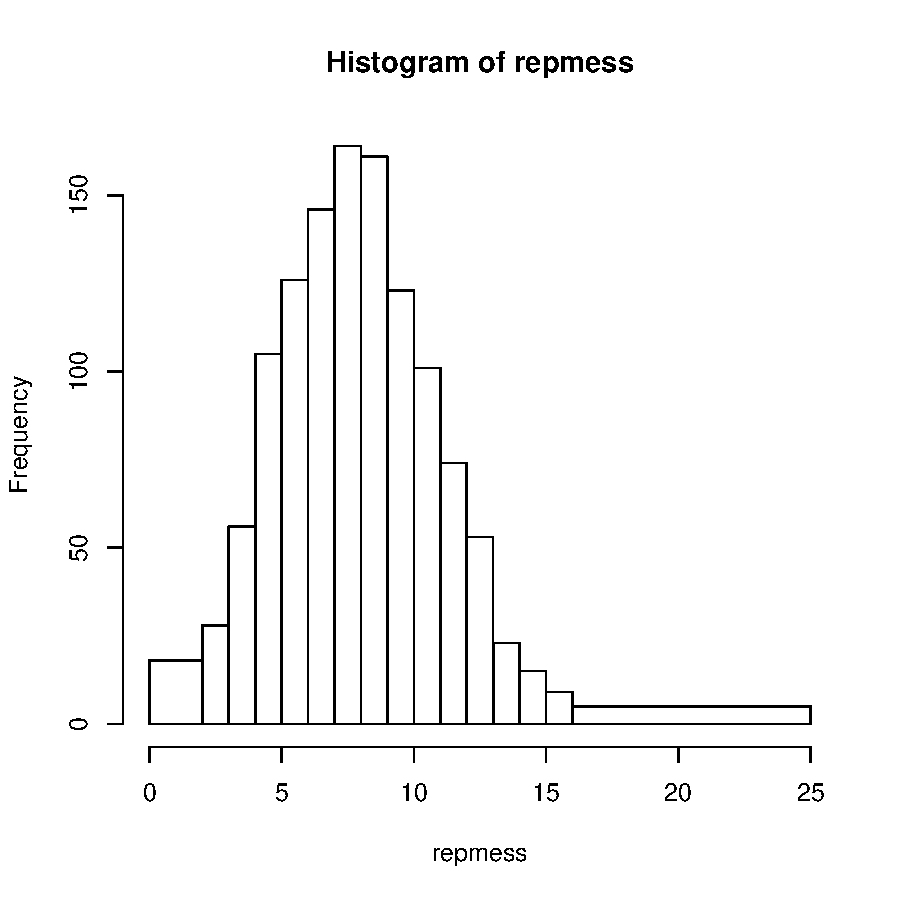
\includegraphics{sw10_1-003}

\subsection{c}
\begin{Schunk}
\begin{Sinput}
> hist(repmess,breaks=c(0,2:16,25),freq=FALSE)
\end{Sinput}
\end{Schunk}
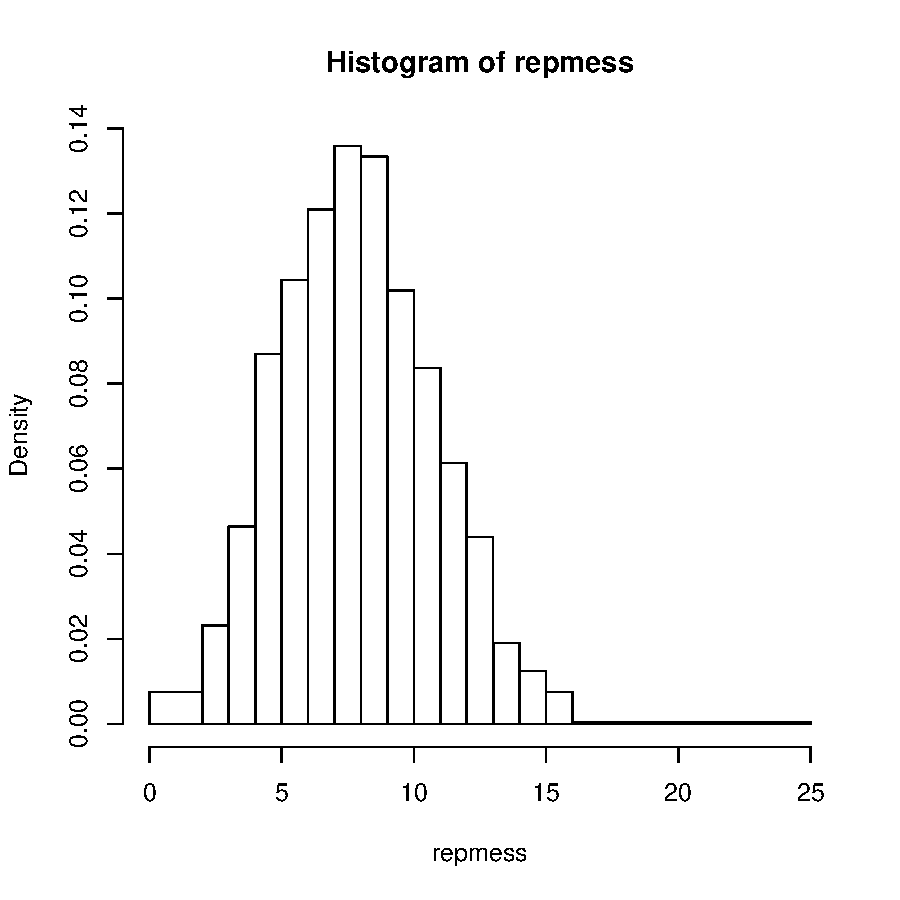
\includegraphics{sw10_1-004}

\subsection{d}
\begin{Schunk}
\begin{Sinput}
> plot(anzzer,anzexp/(sum(anzexp)),type='h')
\end{Sinput}
\end{Schunk}
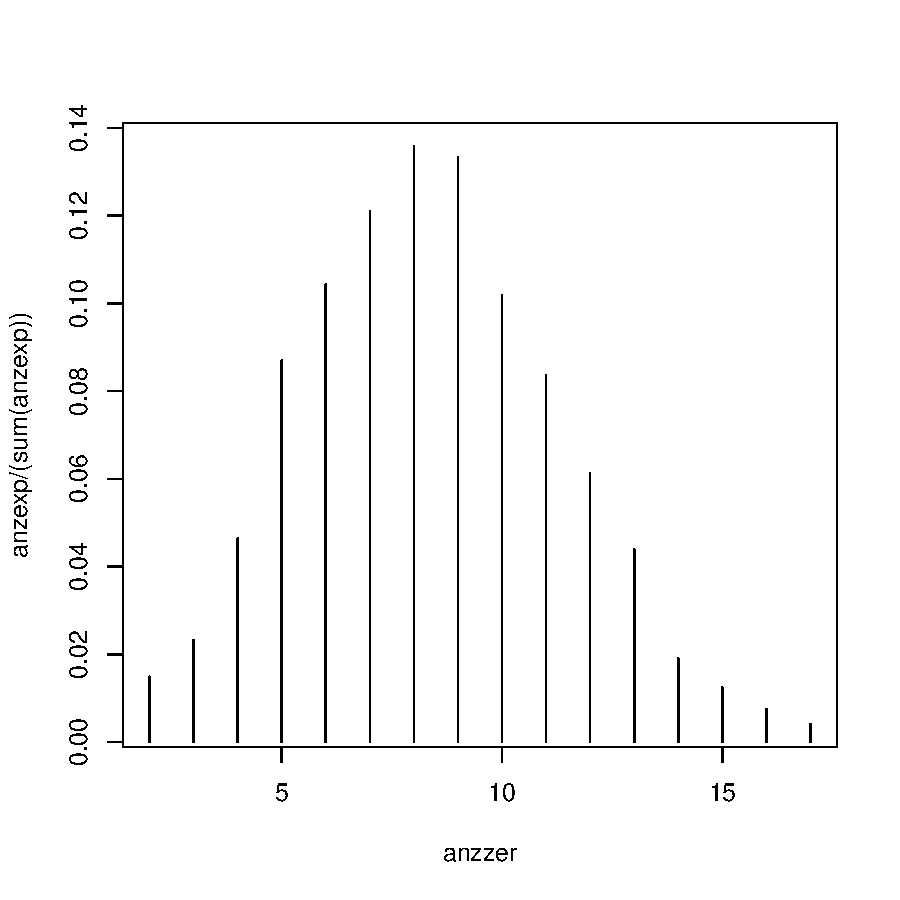
\includegraphics{sw10_1-005}

\subsection{e}
\begin{Schunk}
\begin{Sinput}
> plot(anzzer,anzexp/(sum(anzexp)),type='h')
> meanmess=mean(repmess)
> abline(v=meanmess,col='red')
> sdmess=sd(repmess)
> abline(v=meanmess+sdmess,col='green')
> abline(v=meanmess-sdmess,col='green')
\end{Sinput}
\end{Schunk}
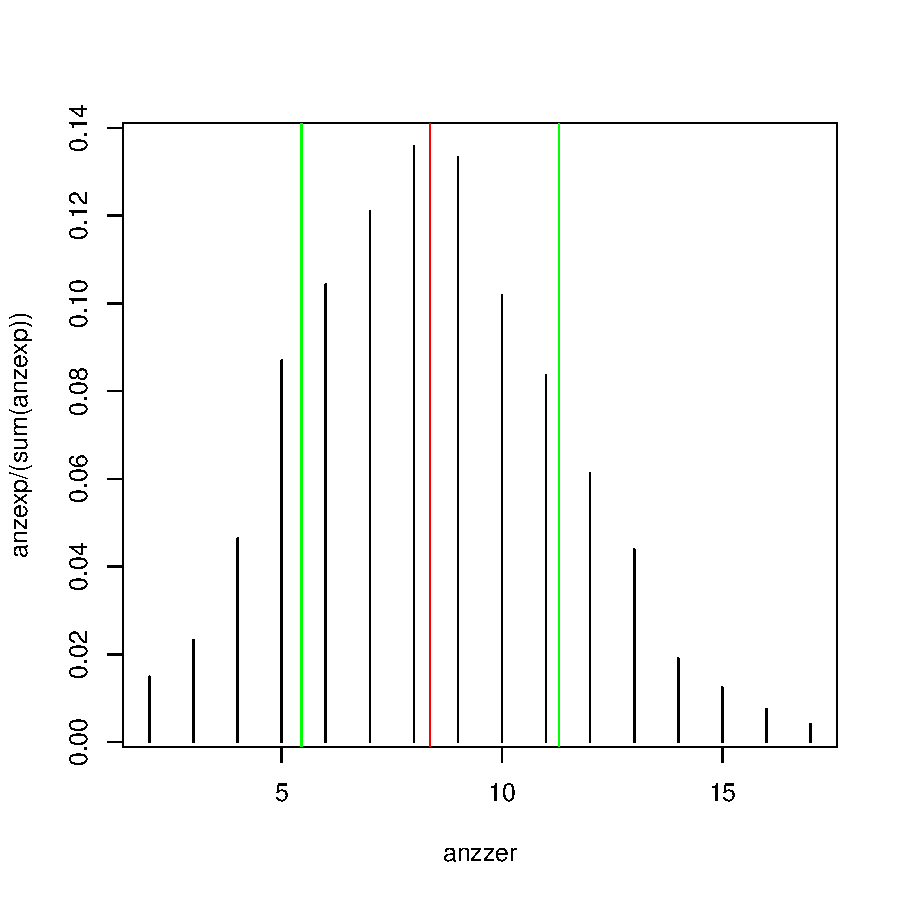
\includegraphics{sw10_1-006}

\subsection{f}
\begin{Schunk}
\begin{Sinput}
> anzexpsum=cumsum(anzexp);
> plot(anzzer,anzexpsum/(sum(anzexp)),type='s')
\end{Sinput}
\end{Schunk}
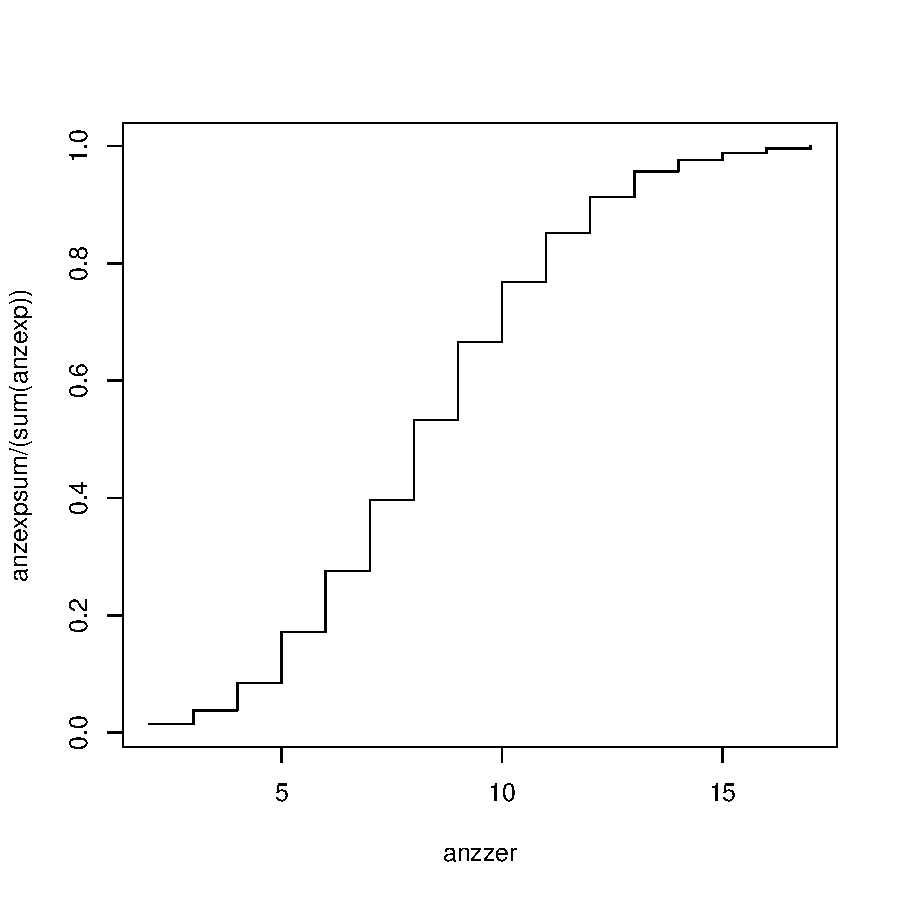
\includegraphics{sw10_1-007}

\subsection{g}
Poissonverteilung mit Lambda = Mittelwert (siehe e)
\begin{Schunk}
\begin{Sinput}
> plot(0:30,dpois(x=0:30,lambda=meanmess),type='h')
> abline(v=meanmess,col='red')
> abline(v=meanmess+sqrt(meanmess),col='green')
> abline(v=meanmess-sqrt(meanmess),col='green')
\end{Sinput}
\end{Schunk}
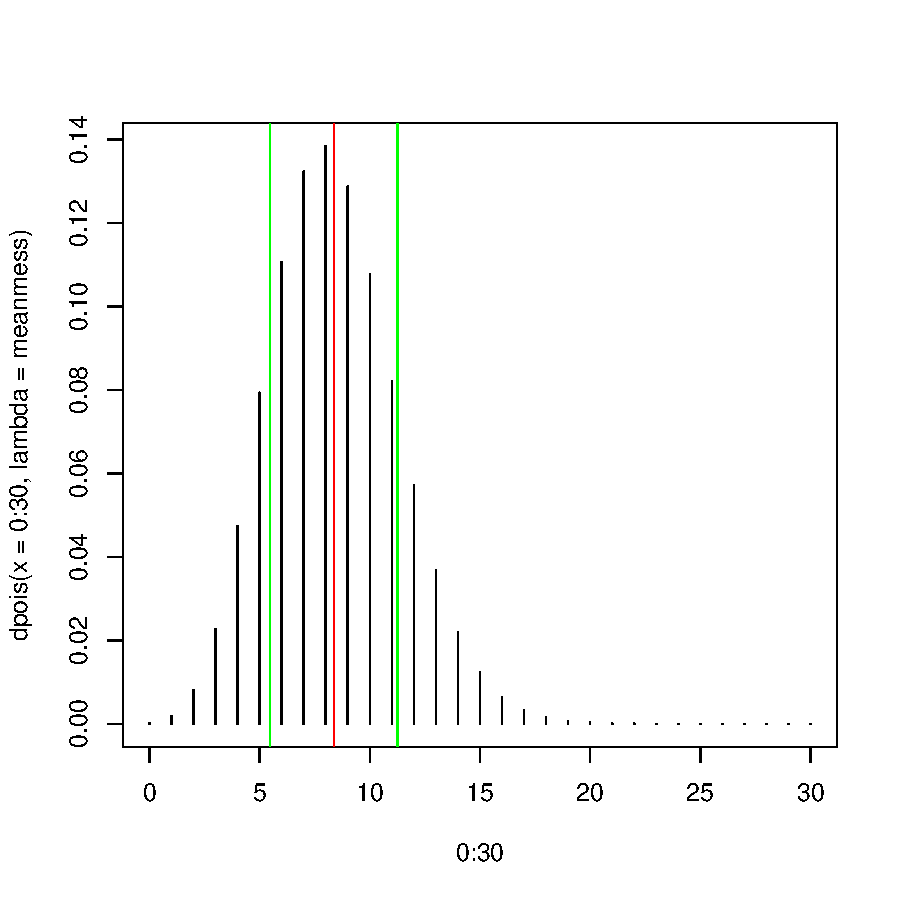
\includegraphics{sw10_1-008}

\subsection{h}
\begin{Schunk}
\begin{Sinput}
> 1e6*(1-ppois(q=19,lambda=meanmess))
\end{Sinput}
\begin{Soutput}
[1] 442.8934
\end{Soutput}
\end{Schunk}

\subsection{i}
\begin{Schunk}
\begin{Sinput}
> plot(0:30,dnorm(x=0:30,mean=meanmess,sd=sqrt(meanmess)),type='h')
\end{Sinput}
\end{Schunk}
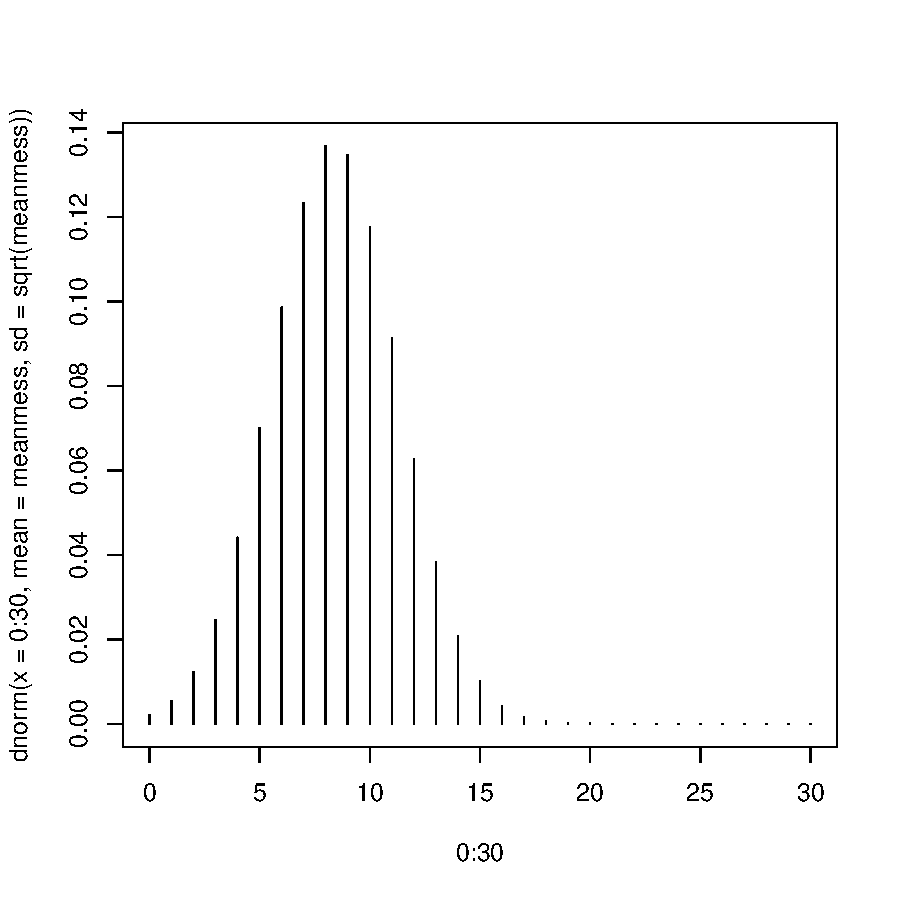
\includegraphics{sw10_1-010}

\subsection{j}
\begin{Schunk}
\begin{Sinput}
> plot(0:300,dexp(x=seq(from=0,to=30,by=0.1),rate=1/meanmess),type='h')
\end{Sinput}
\end{Schunk}
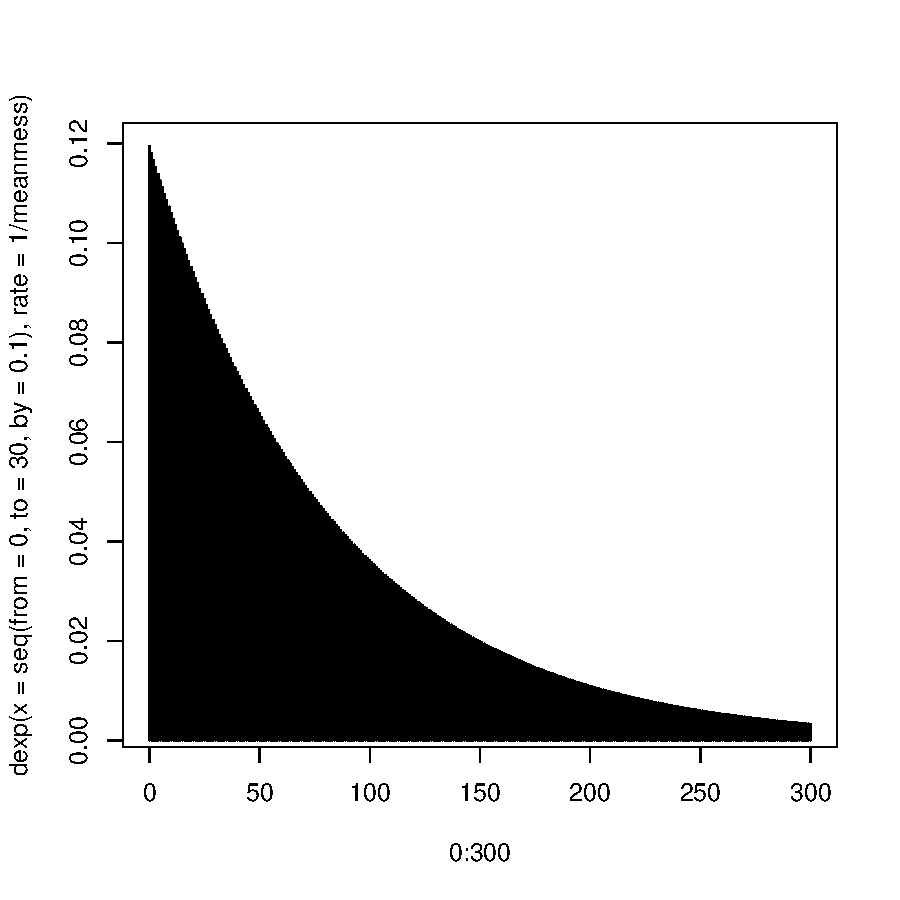
\includegraphics{sw10_1-011}

\subsection{k}
\begin{Schunk}
\begin{Sinput}
> plot(0:300,dexp(x=seq(from=0,to=30,by=0.1),rate=1/meanmess),type='h')
> abline(v=meanmess*10,col='red')
> abline(v=2*meanmess*10,col='green')
\end{Sinput}
\end{Schunk}
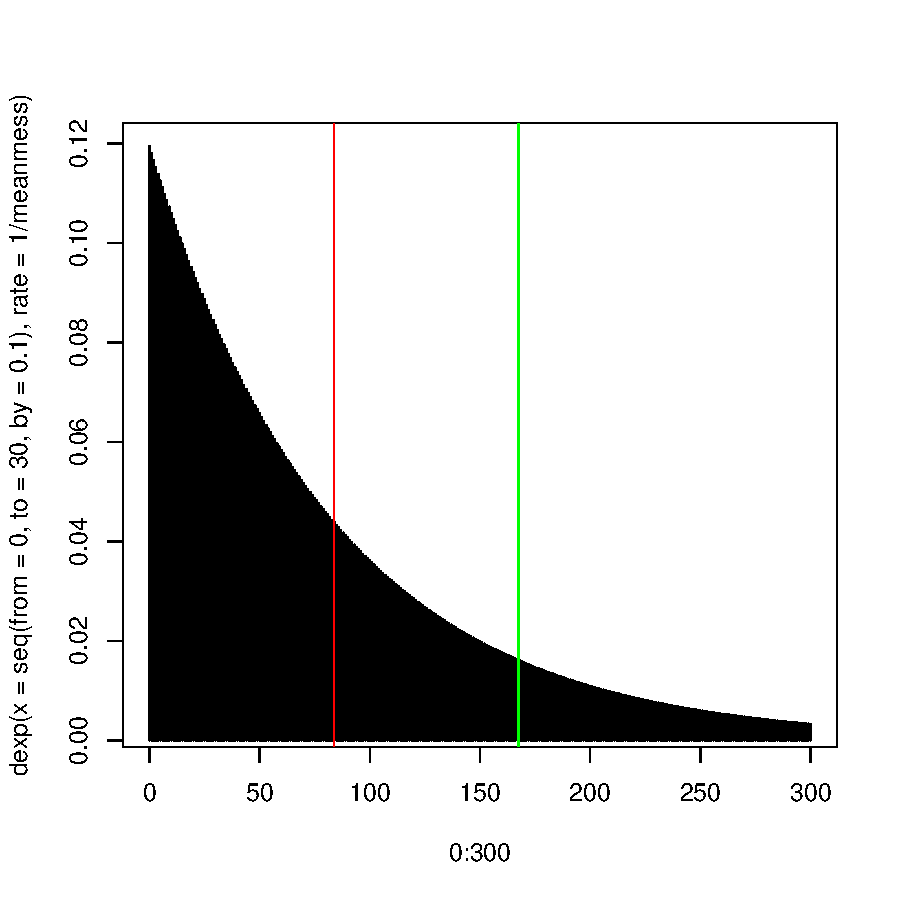
\includegraphics{sw10_1-012}

\subsection{l}

